\documentclass[11pt]{dmathesis}

%% Load the packages to be used.
%%
%% packages.tex - User defined packages for edengths.tex
%%
%% Copyright (C) 2010-2021 Mathew Topper <damm_horse@yahoo.co.uk>
%%
%%   ABOUT
%%
%% This file contains the user defined packages for a Latex2e template which
%% corresponds to the regulations regarding layout of a thesis submitted within
%% the University of Edinburgh.

%%%% PACKAGES AUTOMATTICALLY PROVIDED BY CLASS 
%%%%
%%%%  (No need to reload.  Options can be provided to these packages using the
%%%%   \PassOptionsToPackage command as per example at end.)

%% ifthen     -   Provides simple boolean commands

%% ifpdf      -   Detects whether pdflatex is being used.

%% graphicx   -   Allows inclusion of graphics in eps or jpg/pdf format

%% geometry   -   A more modern way of setting the page margins.
%%                'report' class options are passed automatically.

%% setspace   -   Define line spacing

%% appendix   -   Required for appendices

%% ae         -   Nicer pdf output using T1 fonts

%% fontenc    -   T1 encoding stops some errors for unknown fonts

%% titlesec   -   Custom chapter titles and page headers

%% caption    -   Custom formatting of captions

%% subcaption -   Use subfigures in captions and formatting of such.

%% tocloft    -   Allow modifications to the table of contents and lists

%% mathptmx   -   Option 'msfonts' to use these alternative font packages.
%% helvet         Note: you could add your own font packages in this file.

%% showlabels -   Print labels on the page if 'labels' option is given.

%% hyperef    -   Put clickable links into the document

%% hypcap     -   Links to figures show the figures rather than just the
%%                caption.

%% xcolor     -   Loaded with option 'dvipsnames' with provides colors for pdf
%%                output. The options auto adjust for pdflatex and hyperref.
%%                See http://en.wikibooks.org/wiki/LaTeX/Colors for colours.

%%%%%%%%%%%%%%%%%%%%%%%%%%%%%%%%%%%%%%%%%%%%%%%%%%%%%%%%%%%%%%%%%%%%%%%%%%
%%%%%          Put ADDITIONAL packages you want to use here           %%%%
%%%%%%%%%%%%%%%%%%%%%%%%%%%%%%%%%%%%%%%%%%%%%%%%%%%%%%%%%%%%%%%%%%%%%%%%%%

%% Typset URLs properly. This package does automatic breaking of long URLs.
%% If you're using hyperref you dont need this but you might need the
%% 'breakurl' package depending on your compilation route.
%% Note: 'breakurl' must be the last package (which is normally 'hyperref').
\usepackage[hyphens]{url} 

%% AMS Math Packages
\usepackage{amsmath}
\usepackage{amssymb}
\usepackage{amsthm}

%% Fancy chemical symbols (Might require installation)
\usepackage[version=4]{mhchem}

%% SI units
\usepackage{siunitx}
\DeclareSIUnit\molar{\mole\per\cubic\deci\metre}
\DeclareSIUnit\Molar{\textsc{m}}
\DeclareSIUnit\calorie{cal}
\sisetup{detect-all}

%% Better fractions ie 1/2 with diagonal slash
\usepackage{nicefrac}

%% Nicer tables
\usepackage{booktabs}

%% Citations
%\usepackage[natbibapa]{apacite}
\usepackage[
  natbib=true,
  backend=biber,
  doi=false,
  isbn=false,
  url=false,
  date=year,
  style=authoryear,
  citestyle=authoryear,
  minnames=1,
  maxnames=2,
  minbibnames=1,
  maxbibnames=99,
  giveninits=true]{biblatex}
\addbibresource{bib/arin-all.bib}
\bibliography{bib/arin-all}

%% Proper hyphenation
\usepackage[british]{babel}

%% Rotating
\usepackage{pdflscape}

%% Paragraph control
\usepackage[defaultlines=4,all]{nowidow}


%%%%%%%%%%%%%%%%%%%%%%%%%%%%%%%%%%%%%%%%%%%%%%%%%%%%%%%%%%%%%%%%%%%%%%%%%%
%%%%%             Pass OPTIONS to packages you want here              %%%%
%%%%%%%%%%%%%%%%%%%%%%%%%%%%%%%%%%%%%%%%%%%%%%%%%%%%%%%%%%%%%%%%%%%%%%%%%%

%% Pass natbib the option 'numbers'
% \PassOptionsToPackage{numbers}{natbib}




%% The following is to control the format of your thesis.
\input{format}

%% The following adds user definitions.
\input{defs}

%% Set the path for diagrams.
\graphicspath{{../diagrams/chapter_2/}{../diagrams/chapter_3/}{../diagrams/chapter_4/}
{../diagrams/chapter_5/}{../diagrams/chapter_6/}{../diagrams/appendix/}}

%% Print equation labels next to equation numbers. Use final option to stop
\usepackage[inner]{showlabels}
%\usepackage[notref,notcite]{showkeys}

%\renewcommand{\showlabelfont}{\small\upshape}

\begin{document}

%% Front pages of thesis.
\input{frontpage}

%% Development table of contents
% \newpage
% \pagenumbering{roman}
% \setcounter{page}{1}
% \tableofcontents

%% Main text.
\newpage
\pagenumbering{arabic}
\setcounter{page}{1}

\chapter{Some Simple Text}

\section{Using some `natbib' Citations}

The following paragraph demonstrates some simple text with some citations. The
command
\begin{verbatim}
\citep[see][]{bibtex:key}
\end{verbatim}
puts a citation in parathesis with the word `see' before the
reference itself. The second optional `[~]' puts something after the reference,
such as `chapter 3' as seen in the second citation in the paragraph. Also the
command
\begin{verbatim}
\citet[]{bibtex:key}
\end{verbatim}
will produce an inline citation, i.e., not in parenthesis. Note that a blank
line must be places between paragraphs in the raw latex, e.g.
\begin{verbatim}
Some text in first paragraph.

Some text in second paragraph.
\end{verbatim}

At the beginning of this, I'd like to add a reference by \citet{Afjeh:1986:JoFE}
as it has a junior in it and it's good to see how that formats. Pellentesque id
mi sit amet mauris elementum sagittis eget at neque. Quisque id sapien magna, et
pharetra enim. Aenean congue turpis et libero faucibus vitae vulputate erat
facilisis. Pellentesque iaculis orci a nisl scelerisque quis accumsan sem
viverra. In nec risus dolor, vitae adipiscing erat
\citep[see][]{Solomon:2007:CUP} pellentesque id mi sit amet mauris elementum
sagittis eget at neque. Proin tincidunt sollicitudin sagittis. Pellentesque id
mi sit amet mauris elementum sagittis eget at neque. Quisque id sapien magna, et
pharetra enim. Aenean congue turpis et libero faucibus vitae vulputate erat
facilisis. Pellentesque iaculis orci a nisl scelerisque quis accumsan sem
viverra. In nec risus dolor, vitae adipiscing erat
\citep[see][]{Jaccard:2005:CUP} pellentesque iaculis orci a nisl scelerisque
quis accumsan sem viverra. In nec risus dolor, vitae adipiscing erat.

\section{Entering and Referencing a Figure}

The next paragraph demostrates a reference to a figure and then a the figure
itself. Note the standard layout for a figure is
\begin{verbatim}
\begin{figure}[htb] % htb is positional preference (here, top, bottom)
  \centering
  \includegraphics[width=some width]{filename without extension}
  \caption{Caption Title}
  \label{fig:label}
\end{figure}.
\end{verbatim}
The reference to the figure is then provided by something like
\begin{verbatim}
figure~\ref{fig:label}.
\end{verbatim}

Lorem ipsum dolor sit amet, consectetur adipiscing elit. Pellentesque id mi sit
amet mauris elementum sagittis eget at neque. Quisque id sapien magna, et
pharetra enim. Aenean congue turpis et libero faucibus vitae vulputate erat
facilisis. Pellentesque iaculis orci a nisl scelerisque quis accumsan sem
viverra. In nec risus dolor, vitae adipiscing erat. Etiam ultrices leo eget arcu
faucibus congue. Nullam eget iaculis mauris. Ut gravida rutrum nisl eget auctor.
Donec sodales enim at massa porta nec mattis est dapibus. Nunc nec vehicula
tellus. Quisque massa tellus, lobortis vel sodales sed, aliquet varius dui.
Proin tincidunt sollicitudin sagittis. Figure~\ref{fig:bottomkutta} shows
something unrelated to this paragraph, but neatly demonstrates how to stick a
figure in and reference it.

\begin{figure}[htb]
  \centering
  %% Because graphicspath was set in edengths.tex you only need to
  %% supply the file name here, i.e. examplepicture (doesn't need the
  %% extension) and not the full path. Just remember to add the path
  %% to \graphicspath{{thispath/}{thatpath/}}
  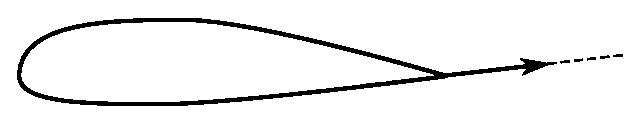
\includegraphics[width=0.3\textwidth]{bottomkutta}
  \caption{Alternative orientations of the wake vortex sheet as it separates
  from the trailing edge of the aerofoil.}
  \label{fig:bottomkutta}
\end{figure}

\section{Quoting Something}

The final paragraph in this chapter illustrates a quote. To do a quote
simply use the enviroment
\begin{verbatim}
\begin{quote}
 The quote text.
\end{quote}.
\end{verbatim}
Note that the edengths class forces quotes to single spacing as the thesis
regulations demand this. Also, there is an inline citation in the next
paragraph.

Lorem ipsum dolor sit amet, consectetur adipiscing elit. Pellentesque id mi sit
amet mauris elementum sagittis eget at neque. Quisque id sapien magna, et
pharetra enim. Aenean congue turpis et libero faucibus vitae vulputate erat
facilisis. Pellentesque \citet[2008]{CCC:2008} iaculis orci a nisl scelerisque
quis accumsan sem viverra. In nec risus dolor, vitae adipiscing erat. Etiam
ultrices leo eget arcu faucibus congue. Nullam eget iaculis mauris. Ut gravida
rutrum nisl eget auctor. Donec sodales enim at massa porta nec mattis est
dapibus. Nunc nec vehicula tellus. Quisque massa tellus, lobortis vel sodales
sed, aliquet varius dui. Proin tincidunt sollicitudin sagittis. 
\begin{quote}
 ``Lorem ipsum dolor sit amet, consectetur adipiscing elit. Pellentesque id mi
sit amet mauris elementum sagittis eget at neque. Quisque id sapien magna, et
pharetra enim. Aenean congue turpis et libero faucibus vitae vulputate erat
facilisis.''
\end{quote}
Lorem ipsum dolor sit amet, consectetur adipiscing elit. Pellentesque id mi sit
amet mauris elementum sagittis eget at neque. Quisque id sapien magna, et
pharetra enim. Aenean congue turpis et libero faucibus vitae vulputate erat
facilisis. Pellentesque iaculis orci a nisl scelerisque quis accumsan sem
viverra. In nec risus dolor, vitae adipiscing erat. Etiam ultrices leo eget arcu
faucibus congue. Nullam eget iaculis mauris. Ut gravida rutrum nisl eget auctor.
Donec sodales enim at massa porta nec mattis est dapibus. Nunc nec vehicula
tellus. Quisque massa tellus, lobortis vel sodales sed, aliquet varius dui.
Proin tincidunt sollicitudin sagittis. 

\chapter{Another Chapter}

\section{The first section}

Note that all section and chapter titles should use lower case except
for the first character of the first word. Here is a reference to a
paper~\cite{apaper}. Figure~\ref{fig:picture} is a weird picture.

\begin{figure}[h]
  \centering
  %% Because graphicspath was set in edengths.tex you only need to
  %% supply the file name here, i.e. examplepicture (doesn't need the
  %% extension) and not the full path. Just remember to add the path
  %% to \graphicspath{{thispath/}{thatpath/}}
  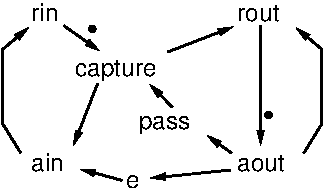
\includegraphics[width=2in]{examplepicture}
  \caption[Long caption and \textit{some italics} to see what happens]%
  {This is an example of pdf with a very long caption and \textit{some italics}
  to see what happens and it should see what happens over two lines.}
\label{fig:picture}
\end{figure}

\subsection{A subsection}

Lorem ipsum dolor sit amet, consectetur adipiscing elit. Maecenas nec orci 
lacus, ac sollicitudin tortor. Maecenas rutrum vestibulum rhoncus. Vestibulum 
non ligula nibh. Cum sociis natoque penatibus et magnis dis parturient montes, 
nascetur ridiculus mus. Phasellus egestas sodales lacus, ac scelerisque nulla 
venenatis sed. Ut elementum turpis ac lacus consectetur consequat. Sed at est 
eros. Praesent erat velit, dictum id adipiscing eu, ultrices vel nisi. Nullam 
at nisl ut est posuere commodo tincidunt eget nisl. Integer id erat non metus 
adipiscing dignissim quis sed enim. Curabitur viverra lobortis eleifend. Proin 
vestibulum nunc eu augue dapibus quis porttitor ipsum rhoncus. Duis tortor 
tellus, suscipit sit amet ornare id, lacinia sed lacus. Ut in molestie ligula. 
Praesent euismod lectus vitae arcu malesuada tempus. Aliquam pharetra 
tincidunt augue in eleifend. Curabitur porttitor vulputate quam, ut fringilla 
mauris porta eu. Curabitur sodales, felis non vestibulum feugiat, urna diam 
bibendum purus, ac scelerisque massa eros sit amet ipsum. In elementum laoreet 
aliquam.

\subsubsection{A subsubsection}

Aliquam eget sapien tellus, sed rutrum leo. Vestibulum et quam sit amet dolor 
gravida sagittis. Aenean dapibus urna a nibh sollicitudin pharetra. Sed nisi 
augue, vehicula sed tristique facilisis, lacinia ut augue. Nam quis tempor mi. 
Vestibulum lorem leo, aliquet at sollicitudin vitae, fringilla id odio. Aenean 
a orci odio. Mauris tincidunt eros ac libero suscipit molestie. Donec feugiat 
turpis a urna suscipit in pellentesque magna pretium. Vivamus eget nunc vitae 
nunc ultricies tincidunt. Duis dictum eros et lorem auctor id ullamcorper diam 
commodo. Pellentesque quis dolor nec urna vestibulum pellentesque. Donec 
luctus mi ut nisi hendrerit pulvinar. Donec fringilla, lectus vitae accumsan 
sollicitudin, sem metus mollis risus, nec laoreet ante arcu ut augue.

\subsection{Another subsection}

Table~\ref{tab:atable} is an example of a~\footnote{this is a
footnote} simple table.

\begin{table}[htb]
\begin{center}
\begin{tabular}{|c|c|c|}
\hline
1.0 & 2.0 & 3.0 \\
\hline
4.0 & 5.0 & 6.0 \\
\hline
\end{tabular}
\caption{A table}
\label{tab:atable}
\end{center}
\end{table}


\section{Another section}

This is a long and boring paragraph for the purpose of testing the
spacing between paragraphs and the use or otherwise of indentation. I
think a space between paragraphs and without the first line indented
is somewhat easier to read than no space between paragraphs and with
the first line indented.

Another equally exciting paragraph, one two three four five six seven
eight nine ten eleven twelve thirteen fourteen fifteen sixteen
seventeen eighteen nineteen twenty and so on.

\begin{equation} \label{eqn:dct}
z(k,l) = \frac{2}{N} \alpha(k) \alpha(l) \sum_{m=0}^{N-1} \sum_{n=0}^{N-1}
         x(m,n) \cos \frac{ (2m+1) \pi k}{2N} \cos \frac{ (2n+1) \pi l}{2N}
\end{equation}

\begin{equation} \label{eqn:idct}
x(m,n) = \frac{2}{N} \sum_{k=0}^{N-1} \sum_{l=0}^{N-1}
         \alpha(k) \alpha(l) z(k,l)
\end{equation}

\begin{quotation}
This is a quotation, another equally exciting paragraph, one two three
four five six seven eight nine ten eleven twelve thirteen fourteen
fifteen sixteen seventeen eighteen nineteen twenty and so on. Just
checking it is single spaced.
\end{quotation}

\section{Section with a landscape image}

\Autoref{fig:landscape} is an image on a landscape orientated page with
the header removed and a simple footer added.

\begin{landscape}
\thispagestyle{plain} % Remove this line for normal headers
\begin{figure}[p]
  \centering
    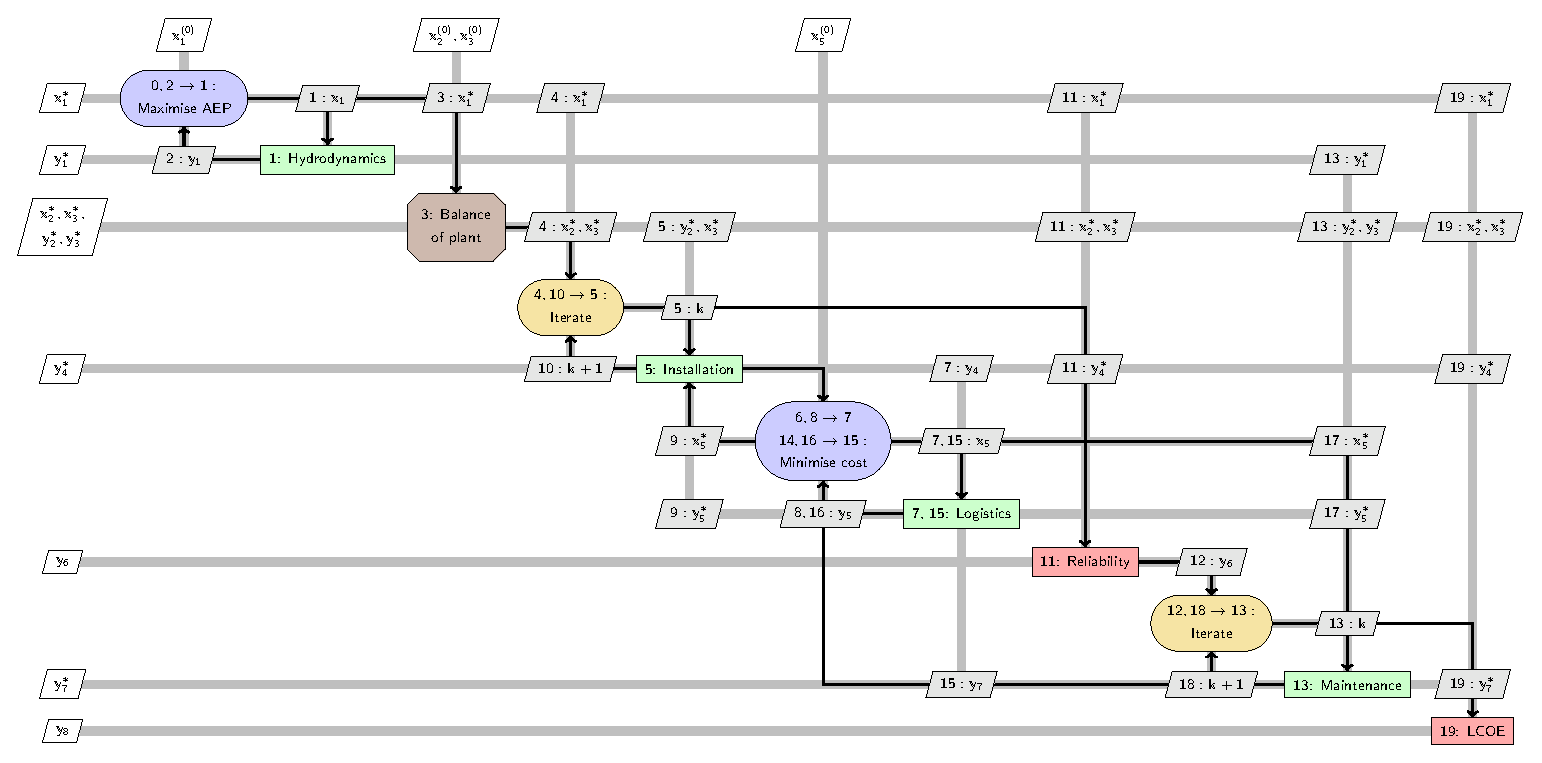
\includegraphics[width=\linewidth]{xdsm_sequential-crop}
    \caption{XDSM diagram. Reproduced from \citep{topper2021}.
    \label{fig:landscape}
}
\end{figure}
\end{landscape}

\include{chapter3}
\include{chapter4}
\include{chapter5}
\include{chapter6}
\include{chapter7}

%% Appendices
\appendix
\noappendicestocpagenum
\addappheadtotoc
\renewcommand{\chaptername}{Appendix}
\renewcommand{\theequation}{\Alph{chapter}.\arabic{equation}}

\input{appendix8}
\input{appendix2}
\input{appendix3}
\input{appendix4}
\input{appendix5}
\input{appendix6}
\input{appendix7}
\input{appendix1}


%% Write out bibliography.
\bibliography{mainrefs}{}
\bibliographystyle{topplainnat}

\end{document}
